\documentclass[12pt]{article}
\usepackage[a4paper,margin=1.25cm]{geometry}
\usepackage{amsmath,amssymb,mathtools}
\usepackage{graphicx}
\usepackage{booktabs}
\usepackage{tabularx}
\usepackage{tikz}
\usepackage[T1]{fontenc}
\usepackage[utf8]{inputenc}
\usepackage[english]{babel}

\setlength{\parindent}{0pt}
\setlength{\parskip}{0.45em}
\setlength{\abovedisplayskip}{5pt plus 1pt minus 1pt}
\setlength{\belowdisplayskip}{5pt plus 1pt minus 1pt}
\setlength{\abovedisplayshortskip}{3pt plus 1pt minus 1pt}
\setlength{\belowdisplayshortskip}{3pt plus 1pt minus 1pt}

\newcommand{\dd}{\,\mathrm{d}}
\newcommand{\e}{\mathrm{e}}
\newcommand{\Sn}{S_n}

\begin{document}

\begin{center}
{\Large\bfseries A sum concentrated at its last few terms}\\[0.35em]
{\large \(\sum(k/n)^k\) and the geometric series with ratio \(1/\mathrm e\)}
\end{center}

\[
\boxed{\displaystyle
\lim_{n\to\infty}\sum_{k=1}^{n}\left(\frac kn\right)^k
=\sum_{j=0}^{\infty}\e^{-j}
=\frac{\e}{\e-1}
=1.5819767\ldots}
\]

\textbf{Overview.}
Count from the top. Writing \(j=n-k\), the terms become
\[
a_{n,j}=\left(1-\frac jn\right)^{n-j},
\]
and for each fixed \(j\),
\[
a_{n,j}=\left(1-\frac jn\right)^{n}\left(1-\frac jn\right)^{-j}
\longrightarrow \e^{-j}\cdot1 .
\]
So the last few terms of the sum converge to the geometric sequence
\(1,\e^{-1},\e^{-2},\dots\), whose total is \(\frac{\e}{\e-1}\). All the
work consists of showing that everything else, the first few terms and
the entire middle, contributes nothing in the limit, uniformly in
\(n\). Two crude geometric bounds suffice: \((k/n)^k\le2^{-k}\) for
\(k\le n/2\) and \((k/n)^k\le \e^{-j/2}\) for \(j\le n/2\).

\section*{1. Setting up a three-block split}

Let
\[
\Sn=\sum_{k=1}^{n}\left(\frac kn\right)^k .
\]
Fix an integer \(M\ge1\) and take \(n>2M\). Substituting \(j=n-k\) in the
top block, split
\[
\Sn=
\underbrace{\sum_{k=1}^{M}\left(\frac kn\right)^k}_{\text{left}}
+\underbrace{\sum_{k=M+1}^{\,n-M-1}\left(\frac kn\right)^k}_{\text{middle}}
+\underbrace{\sum_{j=0}^{M}a_{n,j}}_{\text{right}},
\qquad
a_{n,j}=\left(1-\frac jn\right)^{n-j} .
\tag{1}
\]

\begin{center}
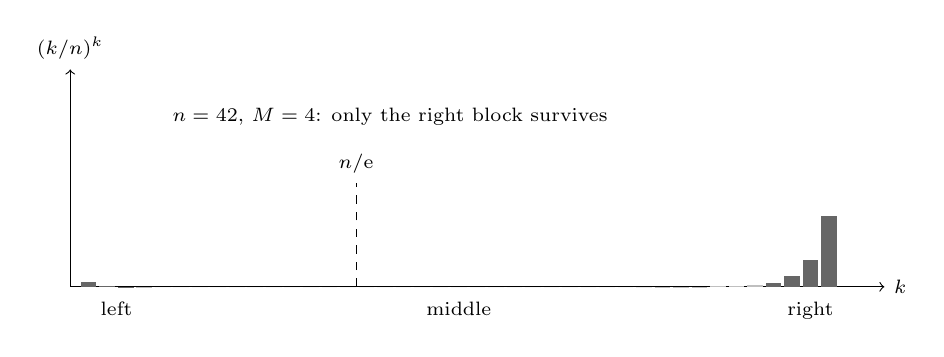
\begin{tikzpicture}[x=0.235cm,y=2.4cm]
\draw[->] (0,0)--(44,0) node[right] {\scriptsize \(k\)};
\draw[->] (0,0)--(0,1.15) node[above] {\scriptsize \((k/n)^k\)};
\foreach \k in {1,...,41}{
  \pgfmathsetmacro{\h}{pow(\k/42,\k)}
  \fill[black!25] (\k-0.42,0) rectangle (\k+0.42,\h);
}
\foreach \k in {38,...,41}{
  \pgfmathsetmacro{\h}{pow(\k/42,\k)}
  \fill[black!60] (\k-0.42,0) rectangle (\k+0.42,\h);
}
\foreach \k in {1,...,4}{
  \pgfmathsetmacro{\h}{pow(\k/42,\k)}
  \fill[black!60] (\k-0.42,0) rectangle (\k+0.42,\h);
}
\draw[dashed] (15.45,0)--(15.45,0.55);
\node[anchor=south] at (15.45,0.55) {\scriptsize \(n/\e\)};
\node[anchor=north] at (2.5,-0.03) {\scriptsize left};
\node[anchor=north] at (21,-0.03) {\scriptsize middle};
\node[anchor=north] at (40,-0.03) {\scriptsize right};
\node[anchor=west] at (5,0.9) {\scriptsize \(n=42\), \(M=4\): only the right block survives};
\end{tikzpicture}
\end{center}

\section*{2. The right block converges term by term}

For \(j\) fixed and \(n\to\infty\),
\[
\left(1-\frac jn\right)^{n}\longrightarrow\e^{-j},
\qquad
\left(1-\frac jn\right)^{-j}\longrightarrow1,
\]
so \(a_{n,j}\to\e^{-j}\). The right block has a fixed number \(M+1\) of
terms, so
\[
\lim_{n\to\infty}\sum_{j=0}^{M}a_{n,j}=\sum_{j=0}^{M}\e^{-j}.
\tag{2}
\]
The tail of this geometric series is
\[
\sum_{j>M}\e^{-j}=\frac{\e^{-M}}{\e-1}\cdot\e ,
\]
which is small for large \(M\).

\section*{3. The left block is \(O(M^2/n)\)}

For \(1\le k\le M\) we have \(\frac kn\le1\), hence
\((k/n)^k\le\frac kn\), and
\[
0\le\sum_{k=1}^{M}\left(\frac kn\right)^k
\le\frac1n\sum_{k=1}^{M}k
=\frac{M(M+1)}{2n}\le\frac{M^2}{n}.
\tag{3}
\]
For each fixed \(M\) this tends to \(0\) as \(n\to\infty\). Note the order
of quantifiers: \(M\) is frozen first, \(n\to\infty\) second, and only at
the very end is \(M\) sent to infinity.

\section*{4. The middle block is uniformly small}

This is the only estimate that must hold uniformly in \(n\). Split the
middle at \(k=n/2\).

\textbf{Lower half, \(M<k\le n/2\).} Here \(\frac kn\le\frac12\), so
\[
\left(\frac kn\right)^k\le\left(\frac12\right)^k=2^{-k},
\qquad\text{hence}\qquad
\sum_{M<k\le n/2}\left(\frac kn\right)^k\le\sum_{k>M}2^{-k}=2^{-M}.
\tag{4}
\]

\textbf{Upper half, \(M<j<n/2\), where \(j=n-k\).} Using
\(\log(1-x)\le-x\),
\[
\left(\frac kn\right)^k
=\left(1-\frac jn\right)^{n-j}
=\exp\!\left[(n-j)\log\left(1-\frac jn\right)\right]
\le\exp\!\left[-\frac{j(n-j)}{n}\right]
\le\e^{-j/2},
\tag{5}
\]
because \(j<\frac n2\) gives \(n-j>\frac n2\) and therefore
\(\frac{j(n-j)}{n}>\frac j2\). Summing,
\[
\sum_{M<j<n/2}\left(\frac kn\right)^k\le\sum_{j>M}\e^{-j/2}
=\frac{\e^{-(M+1)/2}}{1-\e^{-1/2}} .
\tag{6}
\]
Both (4) and (6) are independent of \(n\), and both tend to \(0\) as
\(M\to\infty\). This is exactly what makes the interchange of limits
legitimate.

\section*{5. Conclusion}

Write \(L=\sum_{j\ge0}\e^{-j}=\frac{\e}{\e-1}\). By (1),
\[
\left|\Sn-L\right|
\le\underbrace{\frac{M^2}{n}}_{\text{left, (3)}}
+\underbrace{2^{-M}+\frac{\e^{-(M+1)/2}}{1-\e^{-1/2}}}_{\text{middle, (4),(6)}}
+\left|\sum_{j=0}^{M}a_{n,j}-\sum_{j=0}^{M}\e^{-j}\right|
+\underbrace{\sum_{j>M}\e^{-j}}_{\text{tail}} .
\]
Fix \(\varepsilon>0\). Choose \(M\) so large that the middle bound and the
tail together are \(<\frac\varepsilon2\); this is possible by (4), (6)
and the convergence of \(\sum\e^{-j}\), and the choice does not depend on
\(n\). With \(M\) now fixed, choose \(N\) so large that for \(n\ge N\)
both \(\frac{M^2}{n}\) and the finite-sum discrepancy (which tends to
\(0\) by (2)) are together \(<\frac\varepsilon2\). Then
\(|\Sn-L|<\varepsilon\) for \(n\ge N\), so
\[
\boxed{\displaystyle
\lim_{n\to\infty}\sum_{k=1}^{n}\left(\frac kn\right)^k
=\frac{\e}{\e-1}.}
\]

\section*{6. The refined asymptotics}

The same expansion gives the next order. For fixed \(j\),
\[
\log a_{n,j}=(n-j)\log\left(1-\frac jn\right)
=(n-j)\left(-\frac jn-\frac{j^2}{2n^2}-\cdots\right)
=-j+\frac{j^2}{2n}+O\!\left(\frac{j^3}{n^2}\right),
\]
so \(a_{n,j}=\e^{-j}\bigl(1+\frac{j^2}{2n}+\cdots\bigr)\). Adding the
left block, whose leading term is \(\frac1n\) from \(k=1\), one predicts
\[
\Sn=\frac{\e}{\e-1}+\frac{c}{n}+o\!\left(\frac1n\right),
\qquad
c=1+\frac12\sum_{j\ge0}j^2\e^{-j}
=1+\frac{\e(\e+1)}{2(\e-1)^3},
\tag{7}
\]
using \(\sum_{j\ge0}j^2x^j=\frac{x(1+x)}{(1-x)^3}\) at \(x=\e^{-1}\).
Numerically \(c=1.996142\ldots\), close to but not equal to \(2\).

\begin{center}
\small
\renewcommand{\arraystretch}{1.35}
\begin{tabularx}{0.9\textwidth}{@{}lXX@{}}
\toprule
\(n\) & \(\Sn\) & \(n\left(\Sn-\frac{\e}{\e-1}\right)\) \\
\midrule
\(10\)     & \(1.9080529\) & \(3.26076\) \\
\(100\)    & \(1.6027982\) & \(2.08215\) \\
\(1000\)   & \(1.5839809\) & \(2.00420\) \\
\(10000\)  & \(1.5821764\) & \(1.99695\) \\
\midrule
\(\infty\) & \(1.5819767\) & \(1.99614=c\) \\
\bottomrule
\end{tabularx}
\end{center}

The numerics confirm (7): the rescaled errors descend towards
\(c=1.9961\), the approach itself being \(O(1/n)\).

\section*{7. Where the mass really is}

It is worth locating the maximum of the terms, because it explains why
counting from the top is the right idea and counting from the bottom is
not. Writing \(t=k/n\),
\[
\log\left(\frac kn\right)^k=k\log\frac kn=n\,t\log t,
\]
and \(t\log t\) is minimised at \(t=\e^{-1}\) with value \(-\e^{-1}\).
So the \emph{smallest} term sits near \(k=n/\e\), where it is of size
\(\e^{-n/\e}\), exponentially negligible, and the terms grow
monotonically towards both ends. At the left end they are small because
\(k\) is small; at the right end \((k/n)^k\) approaches \(1\). Hence the
sum is a two-sided affair with a vanishing valley in between, and only
the right end carries mass of order \(1\).

\begin{center}
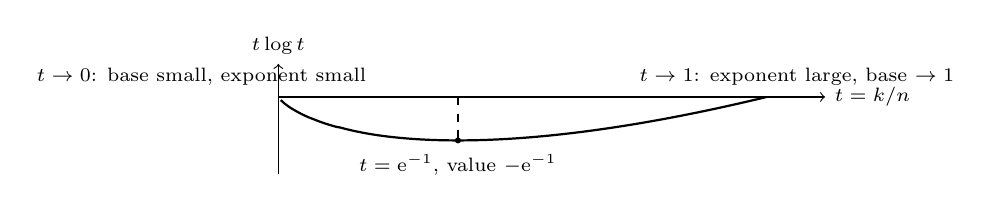
\begin{tikzpicture}[x=6.2cm,y=1.5cm]
\draw[->] (0,0)--(1.12,0) node[right] {\scriptsize \(t=k/n\)};
\draw[->] (0,-0.65)--(0,0.28) node[above] {\scriptsize \(t\log t\)};
\draw[thick,samples=140,domain=0.005:1,smooth] plot (\x,{\x*ln(\x)});
\draw[dashed] (0.3679,0)--(0.3679,-0.3679);
\fill (0.3679,-0.3679) circle (1.1pt);
\node[anchor=north] at (0.3679,-0.40) {\scriptsize \(t=\e^{-1}\), value \(-\e^{-1}\)};
\node[anchor=south west] at (0.72,0.02) {\scriptsize \(t\to1\): exponent large, base \(\to1\)};
\node[anchor=south east] at (0.20,0.02) {\scriptsize \(t\to0\): base small, exponent small};
\end{tikzpicture}
\end{center}

The two ends are not symmetric. At the left end the exponent \(k\) is
small but so is the base, and \((k/n)^k\le\frac kn\to0\): each term
individually vanishes. At the right end the base tends to \(1\) while the
exponent grows like \(n\), and the product \((n-j)\log(1-\frac jn)\)
stabilises at \(-j\): the terms survive. That asymmetry is what makes (3)
cheap and (5) essential, and it is the reason the limit is a geometric
series in \(\e^{-1}\) rather than anything involving the valley at
\(k=n/\e\).

\end{document}
